\documentclass[border = 10pt]{standalone}
\usepackage{tikz}
\usetikzlibrary{calc,positioning,shadows.blur,decorations.pathreplacing}

\tikzset{%
	round/.style = {rounded corners = 2mm}
	}


\begin{document}
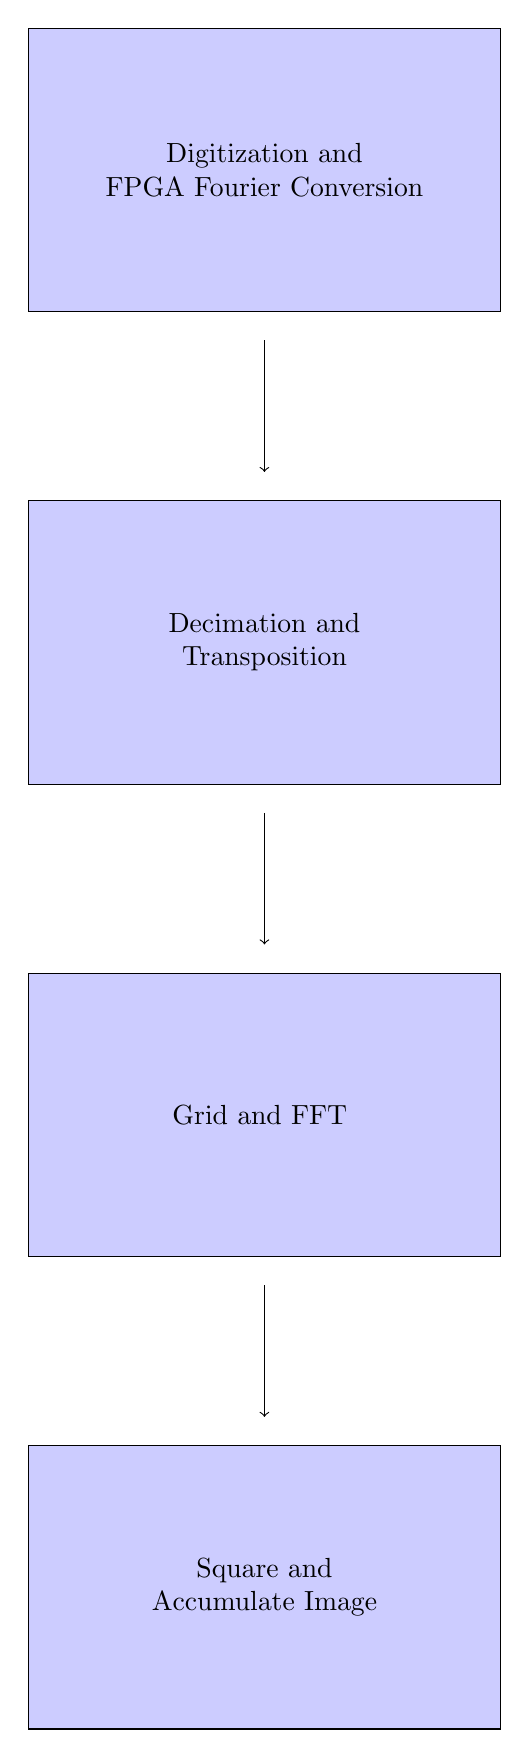
\begin{tikzpicture}[x=1.2cm,y=1.2cm]
  
  \foreach \i in {0,...,3}
  {
    \draw [fill=blue, fill opacity = 0.2] (0,\i*5) -- (5,\i*5) -- (5,\i*5 + 3) -- (0,\i*5+3) -- (0,\i*5);
  }
  \foreach \i in {0,...,2}
  {
    \path (2.5,\i*5 + 3.2) node (y1) {} (2.5,\i*5+4.8) node (y2) {};
    \draw [->] (y2) -- (y1);
  }

  \node at (2.5,16.5) [align=center] { Digitization and \\ FPGA Fourier Conversion };
  \node at (2.5,11.5) [align=center] { Decimation and \\ Transposition};
  \node at (2.5,6.5)  [align=center] { Grid and FFT };
  \node at (2.5,1.5)  [align=center] { Square and \\ Accumulate Image };
\end{tikzpicture}
\end{document}
